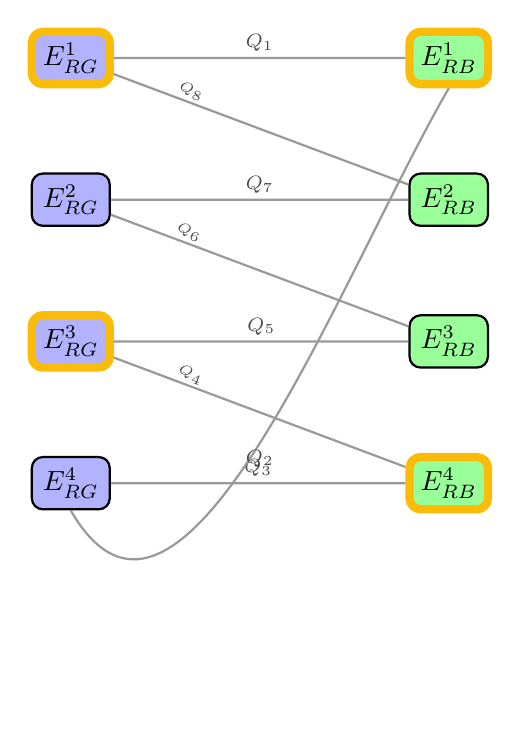
\begin{tikzpicture}[scale=1.2,
    nodeRG/.style={rectangle, rounded corners, draw=black, thick, fill=blue!30, inner sep=4pt, minimum width=24pt, minimum height=16pt},
    nodeRB/.style={rectangle, rounded corners, draw=black, thick, fill=green!40, inner sep=4pt, minimum width=24pt, minimum height=16pt},
    active/.style={draw=yellow!50!orange, line width=3pt}]

    % Left column (RG edges)
    \node[nodeRG, active] (RG1) at (-2, 2.25) {$E_{RG}^1$};
    \node[nodeRG] (RG2) at (-2, 0.75) {$E_{RG}^2$};
    \node[nodeRG, active] (RG3) at (-2, -0.75) {$E_{RG}^3$};
    \node[nodeRG] (RG4) at (-2, -2.25) {$E_{RG}^4$};

    % Right column (RB edges)
    \node[nodeRB, active] (RB1) at (2, 2.25) {$E_{RB}^1$};
    \node[nodeRB] (RB2) at (2, 0.75) {$E_{RB}^2$};
    \node[nodeRB] (RB3) at (2, -0.75) {$E_{RB}^3$};
    \node[nodeRB, active] (RB4) at (2, -2.25) {$E_{RB}^4$};

    % Physical qubits connecting them
    \draw[black!40, thick] (RG1) -- (RB1) node[midway, above, sloped, font=\scriptsize, text=black!70, inner sep=2pt] {$Q_1$};
    \draw[black!40, thick] (RG1) -- (RB2) node[midway, above, sloped, font=\tiny, text=black!70, inner sep=1pt, pos=0.25] {$Q_8$};
    
    \draw[black!40, thick] (RG2) -- (RB2) node[midway, above, sloped, font=\scriptsize, text=black!70, inner sep=2pt] {$Q_7$};
    \draw[black!40, thick] (RG2) -- (RB3) node[midway, above, sloped, font=\tiny, text=black!70, inner sep=1pt, pos=0.25] {$Q_6$};

    \draw[black!40, thick] (RG3) -- (RB3) node[midway, above, sloped, font=\scriptsize, text=black!70, inner sep=2pt] {$Q_5$};
    \draw[black!40, thick] (RG3) -- (RB4) node[midway, above, sloped, font=\tiny, text=black!70, inner sep=1pt, pos=0.25] {$Q_4$};

    \draw[black!40, thick] (RG4) -- (RB4) node[midway, above, sloped, font=\scriptsize, text=black!70, inner sep=2pt] {$Q_3$};
    \draw[black!40, thick] (RG4.south) to[out=-60, in=-120] node[midway, below, font=\scriptsize, text=black!70, inner sep=2pt] {$Q_2$} (RB1.south);

\end{tikzpicture}